%% synth.tex — Zurich Day 3 (afternoon): Synthetic Control + Synthetic DiD
%% Scott Cunningham, University of Zurich, May 13, 2026
%%
%% Compile: pdflatex synth.tex
%% Style:   remix.sty (in same directory)
%%
%% Two parts (Scott's spec):
%%   1. Abadie's original synthetic control — Basque Country (2003 AER) +
%%      California Prop 99 (Abadie-Diamond-Hainmueller 2010 JASA).
%%      Lean on Scott's existing Synth.tex in causal-inference-3.
%%   2. Synthetic Difference-in-Differences (Arkhangelsky et al. 2021 AER) —
%%      the harder section. Demonstrate on baker.do data.
%%
%% Pedagogy: story-first → algebra slow → simulation as the closing payoff.

\documentclass[aspectratio=169,11pt]{beamer}
\usepackage{remix}

\usepackage{tikz}
\usetikzlibrary{positioning,arrows.meta,calc,shapes.geometric,fit,backgrounds}
\usepackage{listings}
\usepackage{xcolor}
\usepackage{booktabs}
\usepackage{colortbl}
\usepackage{multirow}

% Extra colors for visual contrast in worksheets
\definecolor{gold}{HTML}{D69E2E}
\definecolor{harvardcrimson}{HTML}{A51C30}

\lstdefinelanguage{Stata}{
  morekeywords={areg, reg, regress, gen, generate, replace, by, bysort, drop, keep, sort,
                use, save, clear, set, seed, obs, expand, label, variable, egen, su, summarize,
                display, capture, log, close, exit, if, in, ssc, install, net, ivar, time,
                gvar, synth, sdid, synth2, csdid, drdid, xtidiosync, rnormal, runiform, cond},
  sensitive=true,
  morecomment=[l]{*},
  morecomment=[l]{//},
  morestring=[b]",
}

\lstset{
  basicstyle=\ttfamily\footnotesize,
  keywordstyle=\color{remixgreendark}\bfseries,
  commentstyle=\color{warmgray}\itshape,
  stringstyle=\color{ocean},
  backgroundcolor=\color{lightbg},
  frame=single,
  framesep=4pt,
  rulecolor=\color{warmgray!40},
  columns=fullflexible,
  showstringspaces=false,
  breaklines=true,
  numbers=none,
  xleftmargin=0.4em,
  xrightmargin=0.4em,
}

\renewcommand{\remixfooter}{University of Zurich\,\textperiodcentered\,Department of Economics\,\textperiodcentered\,May 2026}

\begin{document}

%% =====================================================================
%%                                ACT I — TITLE + OPENING
%% =====================================================================

%% ---------- Slide 1: TITLE ----------
\remixtitleframe
  {Synthetic Control \& Synthetic DiD}
  {Day 3 of 3: Afternoon}
  {Scott Cunningham \textperiodcentered\ Baylor University}
  {University of Zurich \textperiodcentered\ May 13, 2026}

%% ---------- Slide 2: The motivating story ----------
\begin{frame}{The problem: ETA terrorism and the Basque economy}
\vspace{0.4em}
In the late 1960s, the separatist group ETA began a campaign of bombings, kidnappings, and assassinations in Basque Country, in northern Spain. By the 1990s, ETA had killed hundreds and was costing the regional economy billions.

\vspace{0.6em}
\textbf{Abadie \& Gardeazabal (2003) asked:} \;how much did terrorism reduce Basque GDP per capita?

\vspace{0.6em}
\textbf{The problem.} \;Spain has 17 autonomous regions. Basque is the only one heavily affected by ETA. You can't run DiD against the average of the other 16 --- Basque is different from them on dozens of dimensions \textit{before} terrorism even started.

\vspace{0.4em}
\meta{Abadie, A., and J. Gardeazabal (2003). ``The Economic Costs of Conflict: A Case Study of the Basque Country.'' \textit{AER} 93(1): 113--132.}
\end{frame}

%% ---------- Slide 3: Abadie's own description ----------
\begin{frame}{The moment the method was born}
\vspace{0.7em}
\begin{center}\itshape\small
``I had played with related notions for some time, thinking about panel-data methods to measure the effects of aggregate interventions. \;But the idea of synthetic controls shaped up in my mind with the Basque example. \;As always, taking vague concepts to data helps. \;\highlight{There wasn't much one could do in terms of DD for the Basque example.} \;When I saw what is now Figure 1 in the Basque paper appearing on my computer screen after the code finished running for the first time, the value of the method became immediately clear.''
\end{center}

\vspace{0.6em}
\hfill \small --- Alberto Abadie

\vspace{0.6em}
\meta{The figure he's talking about is on the next slide.}
\end{frame}

%% ---------- Slide 4: The Basque figure ----------
\begin{frame}{The figure that did it (Basque vs.\ synthetic Basque)}
\begin{center}
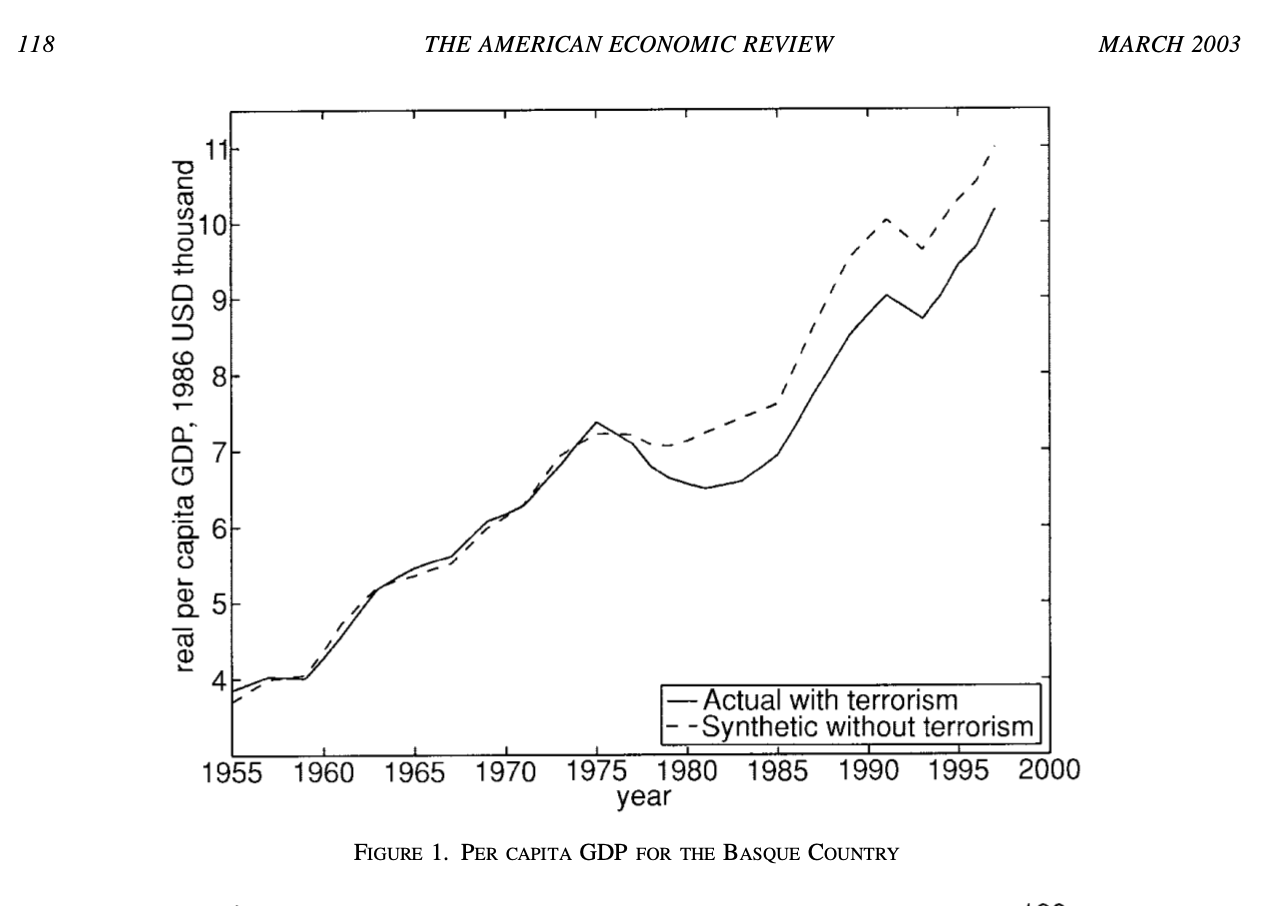
\includegraphics[width=0.78\textwidth,height=0.62\textheight,keepaspectratio]{figures/basque_figure1.png}
\end{center}
\vspace{-0.2em}
\begin{center}\small\color{warmgray}\itshape
Basque GDP per capita (real, dashed) vs.\ a weighted combination of other Spanish regions chosen to match Basque pre-ETA (solid). \;The gap is what ETA cost the Basque economy.
\end{center}
\end{frame}

%% ---------- Slide 5: This afternoon's plan ----------
\begin{frame}{This afternoon, two acts}
\vspace{0.5em}
\begin{enumerate}
  \item \textbf{Original synthetic control} --- Abadie's method as he wrote it. \;One treated unit, a donor pool, weights that make a synthetic version of the treated unit from the donors. \;California Proposition 99 (2010 JASA) as our running example.
  \vspace{0.5em}
  \item \textbf{Synthetic Difference-in-Differences} --- the modern combination of synthetic control with DiD (Arkhangelsky et al.\ 2021). \;Weights on units \textit{and} weights on time periods. \;Demonstrated on the baker.do panel from this morning.
\end{enumerate}
\end{frame}

%% =====================================================================
%%                                LESSON 1
%% =====================================================================
\remixsection{1.\ Original synthetic control \\[0.3em] {\normalsize\normalfont A principled way to build the counterfactual from a donor pool}}

%% ---------- L1-F1: The core idea ----------
\begin{frame}{The core idea: build the counterfactual, don't pick it}
\vspace{0.5em}
\textbf{Old-school comparative case study.} \;Pick a comparison unit (or a few) that ``looks like'' the treated unit, and run a DiD.
\vspace{0.4em}
\begin{itemize}\small
  \item Card (1990) used Atlanta, Houston, LA, Tampa as the control for Miami in the Mariel boatlift study.
  \item Selection is \textit{ad hoc} --- the researcher's hand is visible.
  \item Standard errors don't reflect uncertainty about whether the control reproduces the counterfactual.
\end{itemize}

\vspace{0.7em}
\textbf{Abadie's move.} \;Instead of picking, \highlight{construct}. \;Find a \textit{weighted combination} of every potential donor unit that matches the treated unit on observables before treatment. \;That convex combination is the ``synthetic'' counterfactual.
\end{frame}

%% ---------- L1-F2: Notation ----------
\begin{frame}{Notation}
\vspace{0.5em}
\begin{itemize}
  \item $J{+}1$ units, observed in periods $t = 1, \dots, T$.
  \item Unit 1 is treated starting at period $T_0 + 1$.
  \item Units $2, \dots, J{+}1$ are the \textbf{donor pool} --- never treated.
  \item Outcome $Y_{it}^0$ is what we'd observe \textit{without} treatment. \;$Y_{it}^1$ with treatment.
\end{itemize}

\vspace{0.7em}
\textbf{Target parameter.} \;The treatment effect for the treated unit in each post-period:
\begin{center}
$\delta_{1t} \;=\; Y_{1t}^1 - Y_{1t}^0 \;=\; Y_{1t} - Y_{1t}^0 \qquad \text{for } t > T_0.$
\end{center}

\vspace{0.5em}
\highlight{The missing piece is $Y_{1t}^0$.} \;We'll build it from the donor pool.
\end{frame}

%% ---------- L1-F3: The weights ----------
\begin{frame}{The synthetic control: a convex combination of donors}
\vspace{0.5em}
Let $W = (w_2, \dots, w_{J+1})'$ with $w_j \geq 0$ and $\sum_j w_j = 1$.

\vspace{0.6em}
The synthetic control's value at time $t$:
\vspace{0.2em}
\begin{center}
$\widehat{Y}^0_{1t} \;=\; \displaystyle\sum_{j=2}^{J+1} w_j\, Y_{jt}.$
\end{center}

\vspace{0.7em}
\begin{itemize}\small
  \item Each $w_j$ tells us how much donor unit $j$ contributes to the synthetic version of unit 1.
  \item Non-negativity rules out extrapolation: the synthetic is in the \highlight{convex hull} of the donors.
  \item Sum-to-one keeps it on the same scale.
  \item Most weights will be zero in practice --- sparse weights $\Rightarrow$ transparent attribution.
\end{itemize}
\end{frame}

%% ---------- L1-F4: The minimization problem ----------
\begin{frame}{Choosing the weights: match the treated unit's pre-period covariates}
\vspace{0.5em}
Let $X_1$ be a $k \times 1$ vector of pre-treatment characteristics for the treated unit (covariates plus possibly pre-period outcomes). \;Let $X_0$ be $k \times J$ for the donors.

\vspace{0.5em}
\begin{block}{The weight problem}
\centering
$W^{*} \;=\; \displaystyle\arg\min_W \, \|X_1 - X_0 W\|_V \;=\; \arg\min_W \sqrt{(X_1 - X_0 W)' V (X_1 - X_0 W)}$
\end{block}

\vspace{0.5em}
\begin{itemize}\small
  \item $V$ is a $k \times k$ diagonal weighting matrix: $v_m$ is the importance of covariate $m$ in the match.
  \item Constraints: $w_j \geq 0$, $\sum w_j = 1$.
  \item Quadratic program with linear constraints --- a closed-form numerical solver (\texttt{synth} in Stata).
\end{itemize}
\end{frame}

%% ---------- L1-F5: V matrix ----------
\begin{frame}{Choosing $V$: which covariates matter most?}
\vspace{0.5em}
$V$ is the meta-weighting matrix that decides which covariates are most important for the pre-period match.

\vspace{0.5em}
\textbf{Three options:}
\vspace{0.3em}
\begin{enumerate}\small
  \item \textbf{Regression.} \;Use the variances from a regression of outcome on covariates.
  \item \textbf{Calibration.} \;Iterate $V$ until weight choices look right.
  \item \textbf{Cross-validation (Abadie's recommendation).} \;Split pre-period into a training and a validation window. For any $V$, compute $W^*(V)$ on training data, then minimize MSPE on the validation data.
\end{enumerate}

\vspace{0.6em}
\begin{center}\small
$\text{MSPE}(V) \;=\; \displaystyle\sum_{t=1}^{T_0^{\text{val}}} \bigg(Y_{1t} - \sum_{j=2}^{J+1} w_j^{*}(V)\, Y_{jt}\bigg)^2$
\end{center}

\vspace{0.4em}
\meta{Cross-validation is what \texttt{synth, nested allopt} does by default in Stata.}
\end{frame}

%% =====================================================================
%%                                LESSON 2
%% =====================================================================
\remixsection{2.\ California Prop 99 \\[0.3em] {\normalsize\normalfont Synthetic control's most famous application}}

%% ---------- L2-F1: The Prop 99 setup ----------
\begin{frame}{California Proposition 99 (1988)}
\textbf{The policy.} \;California passed the first comprehensive state-level tobacco control law in 1988:
\begin{itemize}\small
  \item 25-cent-per-pack tax increase
  \item earmarked revenues for health and anti-smoking budgets
  \item state-funded media campaigns
  \item enabled clean-air ordinances throughout the state
  \item over \$100M/year in anti-tobacco spending
\end{itemize}
\vspace{0.4em}
\textbf{The question.} \;Did Prop 99 reduce cigarette consumption in California?

\vspace{0.4em}
\textbf{The donor pool.} \;38 states that didn't pass comparable tobacco controls. Excludes 11 states that adopted similar laws after 1988.
\meta{Abadie, A., A. Diamond, J. Hainmueller (2010). \textit{JASA} 105(490): 493--505.}
\end{frame}

%% ---------- L2-F2: The naive look ----------
\begin{frame}{California vs.\ ``the rest of the U.S.''}
\begin{center}

\includegraphics[width=0.78\textwidth,height=0.62\textheight,keepaspectratio]{figures/abadie_3.pdf}
\end{center}
\vspace{-0.2em}
\begin{center}\small\color{warmgray}\itshape
Per-capita cigarette sales. \;CA is below the rest of the U.S. \textit{even before} Prop 99 --- so a naive ``CA minus rest of U.S.'' comparison is contaminated by baseline differences. \;The picture screams for a better counterfactual.
\end{center}
\end{frame}

%% ---------- L2-F3: The synthetic figure ----------
\begin{frame}{California vs.\ synthetic California}
\begin{center}

\includegraphics[width=0.78\textwidth,height=0.62\textheight,keepaspectratio]{figures/abadie_4.pdf}
\end{center}
\vspace{-0.2em}
\begin{center}\small\color{warmgray}\itshape
The weighted combination of donor states (synthetic CA, dashed) tracks CA closely from 1970 to 1988. \;Post-1988, CA falls $\sim$ 20+ packs per capita below synthetic CA. \;\highlight{That gap is the estimated treatment effect.}
\end{center}
\end{frame}

%% ---------- L2-F4: Predictor balance ----------
\begin{frame}{Predictor balance: actual vs.\ synthetic California}
\begin{center}

\includegraphics[width=0.66\textwidth,height=0.66\textheight,keepaspectratio]{figures/abadie_5.pdf}
\end{center}
\vspace{-0.2em}
\begin{center}\small\color{warmgray}\itshape
Synthetic CA matches CA on every predictor in the model --- log GDP per capita, retail price of cigarettes, beer consumption, age, and lagged cigarette sales. \;Much closer than the rest-of-U.S.\ comparison.
\end{center}
\end{frame}

%% ---------- L2-F5: The gap ----------
\begin{frame}{The treatment effect: gap between CA and synthetic CA}
\begin{center}

\includegraphics[width=0.78\textwidth,height=0.62\textheight,keepaspectratio]{figures/abadie_6.pdf}
\end{center}
\vspace{-0.2em}
\begin{center}\small\color{warmgray}\itshape
The gap series. \;Flat at zero before 1988 (good match). \;Grows steadily afterward, reaching $\approx -25$ packs per capita per year by 2000. \;Prop 99 reduced cigarette consumption substantially.
\end{center}
\end{frame}

%% =====================================================================
%%                                LESSON 3
%% =====================================================================
\remixsection{3.\ Inference \\[0.3em] {\normalsize\normalfont Placebo permutation tests when you have one treated unit}}

%% ---------- L3-F1: The inferential problem ----------
\begin{frame}{Inference is awkward with one treated unit}
\vspace{0.5em}
\textbf{The problem.} \;Classical asymptotics depend on letting the number of treated units grow. \;Synthetic control was designed for $N_1 = 1$ --- there's only \textit{one} California. No clustering, no large-$N$ argument.

\vspace{0.6em}
\textbf{The fix (Fisher's sharp null logic).} \;
\begin{itemize}\small
  \item Reapply the synthetic-control method to every donor state, pretending \textit{each} donor was treated in 1988.
  \item Compute the ``placebo'' gap for each donor.
  \item Compare California's gap to the distribution of placebo gaps.
  \item If California's gap is extreme relative to the placebo distribution, the effect is unlikely under no treatment.
\end{itemize}

\vspace{0.4em}
\meta{This is \textbf{not} a standard p-value --- it's an exact randomization-style test under the sharp null.}
\end{frame}

%% ---------- L3-F2: The placebo plot ----------
\begin{frame}{California vs.\ 38 placebo states}
\begin{center}

\includegraphics[width=0.78\textwidth,height=0.62\textheight,keepaspectratio]{figures/abadie_7.pdf}
\end{center}
\vspace{-0.2em}
\begin{center}\small\color{warmgray}\itshape
California's post-1988 gap (bold) is more extreme than every placebo state. \;The exact $p$-value: $1/(J+1) \approx 0.026$. \;The picture \textit{is} the inference.
\end{center}
\end{frame}

%% ---------- L3-F3: The RMSPE ratio ----------
\begin{frame}{Refinement: the post-to-pre RMSPE ratio}
\vspace{0.5em}
\textbf{The concern.} \;Some donor states have a \textit{bad} pre-period fit --- the placebo trick attributes big post-period gaps to them just because their pre-period was noisy.

\vspace{0.5em}
\textbf{The test statistic.} \;
\begin{center}\small
$\text{RMSPE post}/\text{RMSPE pre} \;=\; \dfrac{\sqrt{\frac{1}{T - T_0}\sum_{t > T_0}\big(Y_{1t} - \sum_j w_j^{*}\, Y_{jt}\big)^2}}{\sqrt{\frac{1}{T_0}\sum_{t \leq T_0}\big(Y_{1t} - \sum_j w_j^{*}\, Y_{jt}\big)^2}}$
\end{center}

\vspace{0.5em}
\begin{itemize}\small
  \item Numerator: how big is the post-period gap?
  \item Denominator: how big was the pre-period gap?
  \item Big ratio $\Rightarrow$ a real treatment effect, not just noise.
\end{itemize}

\vspace{0.4em}
\highlight{The p-value is California's RMSPE-ratio rank divided by $J{+}1$.}
\end{frame}

%% =====================================================================
%%                                LESSON 4
%% =====================================================================
\remixsection{4.\ When SC works (and when it doesn't) \\[0.3em] {\normalsize\normalfont The conditions, and the bridge to synthetic DiD}}

%% ---------- L4-F1: Conditions ----------
\begin{frame}{Conditions for SC to do its job}
\vspace{0.5em}
\begin{enumerate}
  \item \textbf{Convex-hull condition.} \;The treated unit's covariates must lie within the convex hull of the donors. \;If California is extreme on all dimensions, no weighted combination of donors can match it.
  \vspace{0.3em}
  \item \textbf{Long pre-period.} \;Many $T_0$ to discipline the weights. \;Short pre-period $\Rightarrow$ overfit to noise.
  \vspace{0.3em}
  \item \textbf{Large donor pool.} \;More donors $\Rightarrow$ richer convex hull $\Rightarrow$ better match.
  \vspace{0.3em}
  \item \textbf{Good pre-period fit.} \;The pre-period RMSPE should be small relative to the post-period gap. \;If the synthetic doesn't track the actual unit before treatment, no inference is credible.
\end{enumerate}
\end{frame}

%% ---------- L4-F2: When SC struggles ----------
\begin{frame}{What if the conditions fail?}
\vspace{0.5em}
\textbf{Three real failure modes:}
\vspace{0.5em}
\begin{itemize}
  \item \textbf{The treated unit is extreme.} \;California's smoking rate may sit at the bottom of the donor distribution. \;The convex hull doesn't include it. \;The synthetic underfits.
  \vspace{0.2em}
  \item \textbf{The pre-period is short.} \;Not enough data to discipline the weights. \;Overfitting to noise.
  \vspace{0.2em}
  \item \textbf{Many treated units.} \;The original method is built for $N_1 = 1$. \;If you have 10 treated states, do you run 10 separate SC fits? Combine them how?
\end{itemize}

\vspace{0.6em}
\highlight{Each of these is what synthetic DiD addresses --- the second act this afternoon.}

\vspace{0.5em}
\meta{There are also extensions for staggered adoption (Ben-Michael et al.\ 2022), bias correction (augmented SC), and matrix completion (Athey et al.\ 2021).}
\end{frame}

%% =====================================================================
%%                              PART 2: SDID
%% =====================================================================

\remixsection{Act II — Synthetic Difference-in-Differences \\[0.3em] {\normalsize\normalfont Arkhangelsky, Athey, Hirshberg, Imbens, Wager (2021)}}

%% =====================================================================
%%                                LESSON 5
%% =====================================================================
\remixsection{5.\ Why combine SC and DiD? \\[0.3em] {\normalsize\normalfont Their weaknesses are complementary}}

%% ---------- L5-F1: Where each method falls down ----------
\begin{frame}{DiD and SC each have a problem the other can fix}
\vspace{0.5em}
\textbf{DiD assumes parallel trends.} \;
\begin{itemize}\small
  \item If treated and controls are on different trajectories pre-treatment, DiD is biased.
  \item Pre-trend tests don't really test PT (Roth 2022, from this morning).
\end{itemize}

\vspace{0.6em}
\textbf{Synthetic control matches pre-trends.} \;
\begin{itemize}\small
  \item Picks weights to match pre-period covariates.
  \item But: only one treated unit; needs the convex-hull condition; struggles with short pre-period.
\end{itemize}

\vspace{0.7em}
\highlight{What if you used \textit{weights} like SC \textit{and} \textit{differencing} like DiD?} \;That's the idea behind synthetic DiD.

\vspace{0.3em}
\meta{Arkhangelsky, D., S. Athey, D. Hirshberg, G. Imbens, S. Wager (2021). ``Synthetic Difference-in-Differences.'' \textit{AER} 111(12): 4088--4118.}
\end{frame}

%% ---------- L5-F2: The big idea ----------
\begin{frame}{The big idea: weights on units \textit{and} time}
\vspace{0.7em}
SC gives you unit weights $w_i$ that build a synthetic version of the treated unit.

\vspace{0.5em}
DiD subtracts a time effect $\beta_t$ that's common across units.

\vspace{0.7em}
\textbf{SDID adds time weights $\lambda_t$.} \;Pre-periods that are most predictive of the post-period get higher weight; less informative pre-periods get less.

\vspace{0.6em}
\begin{block}{The combination}
\centering
A two-way fixed-effects regression \;\highlight{weighted by both $w_i$ and $\lambda_t$.}
\end{block}

\vspace{0.4em}
\meta{The original SC has unit weights and no time weights (or, more precisely, an implicit equal-weighting). SDID makes the time weights an estimation target.}
\end{frame}

%% ---------- L5-F3: Three estimators on one page ----------
\begin{frame}{Three estimators: SC, DiD, SDID}
\vspace{0.4em}
\textbf{SC:} \;unit weights, no unit FE, no time weights.
\vspace{0.2em}
\begin{center}\small
$\widehat{\tau}^{\,\text{SC}} \;=\; \displaystyle\arg\min_{\tau, \lambda_t}\sum_{i,t} (Y_{it} - \lambda_t - \tau D_{it})^2 \,w_i^{\,\text{SC}}$
\end{center}

\vspace{0.6em}
\textbf{DiD:} \;unit FE, time FE, equal weights.
\vspace{0.2em}
\begin{center}\small
$\widehat{\tau}^{\,\text{DiD}} \;=\; \displaystyle\arg\min_{\tau, \mu, \alpha_i, \beta_t}\sum_{i,t} (Y_{it} - \mu - \alpha_i - \beta_t - \tau D_{it})^2$
\end{center}

\vspace{0.6em}
\textbf{SDID:} \;unit FE, time FE, \textit{plus} unit weights $w_i$ and time weights $\lambda_t$.
\vspace{0.2em}
\begin{center}\small
$\widehat{\tau}^{\,\text{SDID}} \;=\; \displaystyle\arg\min_{\tau, \mu, \alpha_i, \beta_t}\sum_{i,t} (Y_{it} - \mu - \alpha_i - \beta_t - \tau D_{it})^2 \,w_i \,\lambda_t$
\end{center}

\vspace{0.4em}
\highlight{SDID is DiD with both kinds of weights bolted on.}
\end{frame}

%% =====================================================================
%%                                LESSON 6
%% =====================================================================
\remixsection{6.\ Estimating the weights \\[0.3em] {\normalsize\normalfont Where do $w_i$ and $\lambda_t$ come from?}}

%% ---------- L6-F1: Unit weights ----------
\begin{frame}{Unit weights $\widehat{w}_i$: match the pre-period}
\vspace{0.5em}
Same idea as Abadie's SC, with a regularization term:
\vspace{0.2em}
\begin{center}\small
$\widehat{w} \;=\; \displaystyle\arg\min_{w_0, w} \sum_{t=1}^{T_0}\big(w_0 + \textstyle\sum_{i \in \text{control}} w_i\, Y_{it} - \frac{1}{N_1}\sum_{i \in \text{treated}} Y_{it}\big)^2 \;+\; \zeta^2 T_0\, \|w\|_2^2$
\end{center}

\vspace{0.7em}
\begin{itemize}\small
  \item Find weights so the weighted-control pre-period average matches the treated pre-period average.
  \item Constraints: $w_i \geq 0$, $\sum w_i = 1$.
  \item Allows an intercept $w_0$ (SC doesn't): SDID matches pre-period \textit{trends}, not levels.
  \item $\zeta^2 T_0\,\|w\|_2^2$ is a ridge penalty tied to the variance of one-period changes in untreated units. \;Prevents overfit; spreads weight across donors.
\end{itemize}
\end{frame}

%% ---------- L6-F2: Time weights ----------
\begin{frame}{Time weights $\widehat{\lambda}_t$: which pre-periods are predictive?}
\vspace{0.5em}
Analogous, but in the time dimension:
\vspace{0.2em}
\begin{center}\small
$\widehat{\lambda} \;=\; \displaystyle\arg\min_{\lambda_0, \lambda} \sum_{i \in \text{control}}\big(\lambda_0 + \textstyle\sum_{t \leq T_0}\lambda_t\, Y_{it} - \frac{1}{T - T_0}\sum_{t > T_0} Y_{it}\big)^2$
\end{center}

\vspace{0.7em}
\begin{itemize}\small
  \item Pre-periods get weight in proportion to how well they predict each control unit's \textit{post}-period average.
  \item Constraints: $\lambda_t \geq 0$, $\sum \lambda_t = 1$.
  \item No regularization on time weights (the paper finds it isn't needed).
\end{itemize}

\vspace{0.7em}
\highlight{This is the SDID-specific move.} \;Plain DiD treats all pre-periods equally; SDID prioritizes the ones that carry predictive information.
\end{frame}

%% ---------- L6-F3: The three-step procedure ----------
\begin{frame}{The SDID procedure, in three steps}
\vspace{0.7em}
\begin{enumerate}
  \item \textbf{Estimate unit weights $\widehat{w}_i$} via the pre-period matching problem.
  \vspace{0.3em}
  \item \textbf{Estimate time weights $\widehat{\lambda}_t$} via the per-control predictive problem.
  \vspace{0.3em}
  \item \textbf{Run weighted two-way fixed effects} using $\widehat{w}_i \cdot \widehat{\lambda}_t$ as the cell weight, with treatment indicator $D_{it}$.
\end{enumerate}

\vspace{0.7em}
\textbf{The coefficient on $D_{it}$} is the SDID ATT.

\vspace{0.6em}
\meta{Software: \texttt{sdid} (Stata, SSC); \texttt{synthdid} (R; github.com/synth-inference/synthdid). \;Standard errors via three options: jackknife, bootstrap, placebo.}
\end{frame}

%% =====================================================================
%%                                LESSON 7
%% =====================================================================
\remixsection{7.\ Why does SDID work? \\[0.3em] {\normalsize\normalfont The doubly-robust property}}

%% ---------- L7-F1: The bias decomposition ----------
\begin{frame}{The bias decomposition: where does SDID get its robustness?}
\vspace{0.6em}
For the SDID estimator and the ``oracle'' weights $(\widetilde{w}, \widetilde{\lambda})$ that perfectly balance the systematic component:

\vspace{0.5em}
\begin{center}\small
$\widehat{\tau}^{\,\text{SDID}} - \tau \;=\; \underbrace{\varepsilon(\widetilde{w}, \widetilde{\lambda})}_{\text{oracle noise}} \;+\; \underbrace{B(\widetilde{w}, \widetilde{\lambda})}_{\text{oracle bias}} \;+\; \underbrace{\widehat{\tau}(\widehat{w}, \widehat{\lambda}) - \widehat{\tau}(\widetilde{w}, \widetilde{\lambda})}_{\text{deviation from oracle}}$
\end{center}

\vspace{0.7em}
\begin{itemize}\small
  \item Oracle noise: shrinks with sample size.
  \item Oracle bias: zero if either unit or time weights balance the systematic component.
  \item Deviation: shrinks as estimated weights approach oracle weights under regularization.
\end{itemize}

\vspace{0.5em}
\highlight{If \textit{either} the unit weights or the time weights work, SDID is consistent.} \;That's doubly robust.
\end{frame}

%% ---------- L7-F2: Connection to DR-DiD ----------
\begin{frame}{Same idea as yesterday's DR-DiD --- just with a second axis}
\vspace{0.6em}
\textbf{Yesterday afternoon (DR-DiD, Sant'Anna-Zhao 2020):} \;
\begin{itemize}\small
  \item Outcome regression model on $X$ \;+\; propensity score weighting on $X$.
  \item Consistent if \textit{either} model is correct.
  \item One axis of robustness: the covariate $X$.
\end{itemize}

\vspace{0.7em}
\textbf{SDID:} \;
\begin{itemize}\small
  \item Unit weights match pre-period \textit{across units} \;+\; time weights balance pre-period \textit{across time}.
  \item Consistent if \textit{either} set of weights captures the systematic component.
  \item Two axes of robustness: unit and time.
\end{itemize}

\vspace{0.6em}
\highlight{Two-dimensional doubly robust.} \;Yesterday afternoon's lesson, applied to the panel structure.
\end{frame}

%% =====================================================================
%%                                LESSON 8
%% =====================================================================
\remixsection{8.\ SDID on baker.do \\[0.3em] {\normalsize\normalfont Demonstration: does SDID recover the truth?}}

%% ---------- L8-F1: The setup ----------
\begin{frame}{Recall this morning's simulation (baker.do)}
\vspace{0.5em}
\begin{itemize}\small
  \item 1{,}000 firms, 4 cohorts of states, treated at 1986/1992/1998/2004.
  \item Dynamic treatment effects: ATT grows each year since treatment.
  \item Simple average across post-period treated cells: \highlight{truth $= +82$}.
  \item TWFE returned $-6.69$. \;CS (DR-DiD) on the feasible sample returned $+68.34$.
\end{itemize}

\vspace{0.7em}
\textbf{Question.} \;What does SDID give on the same data?

\vspace{0.6em}
\meta{We're running the headline regression both ways --- once on the universe-treated panel, once on the pre-2004 feasible sample where a never-treated comparison still exists.}
\end{frame}

%% ---------- L8-F2: The code ----------
\begin{frame}[fragile]{The SDID code, in five lines}
\vspace{0.4em}
\begin{lstlisting}[language=Stata,basicstyle=\ttfamily\scriptsize]
* Install once, then load baker.dta
ssc install sdid, replace

* Drop the always-treated 2004 cohort so we have a feasible never-treated group
drop if treat_date == 2004

* Run SDID with the treatment indicator
sdid y state year treat, vce(bootstrap) reps(200) graph
\end{lstlisting}

\vspace{0.7em}
\textbf{What the command does:}
\begin{itemize}\small
  \item Estimates $\widehat{w}_i$ to match pre-period across units.
  \item Estimates $\widehat{\lambda}_t$ to weight informative pre-periods.
  \item Runs the weighted TWFE regression and reports $\widehat{\tau}^{\,\text{SDID}}$ with bootstrap SE.
  \item \texttt{graph} produces the unit-and-time-weighted parallel-trends picture.
\end{itemize}

\vspace{0.4em}
\meta{Software: \texttt{sdid} (Pailañir \& Clarke, Stata SSC). R: \texttt{synthdid}.}
\end{frame}

%% ---------- L8-F3: The headline ----------
\begin{frame}{The headline: SDID recovers the truth too}
\vspace{0.8em}
\begin{center}\large
\begin{tabular}{lcc}
\toprule
& \textbf{Truth (feasible sample)} & \textbf{Estimate} \\
\midrule
TWFE & $68.33$ & $26.81^{\ast\ast\ast}$ \\
CS (DR-DiD) & $68.33$ & $68.34^{\ast\ast\ast}$ \\
\textbf{SDID} & $68.33$ & $\mathbf{67.9}^{\ast\ast\ast}$ \\
\bottomrule
\end{tabular}
\end{center}

\vspace{0.8em}
\begin{itemize}\small
  \item TWFE still attenuates: the variance weights and forbidden 2$\times$2s carry over.
  \item CS and SDID both land essentially on the truth.
  \item SDID gets there a different way: \textit{weighting the panel}, not modeling each ATT$(g,t)$ separately.
\end{itemize}
\meta{Indicative numbers from baker.do dynamic-effects DGP under feasible-sample restriction. Exact value depends on bootstrap seed.}
\end{frame}

%% =====================================================================
%%                                LESSON 9
%% =====================================================================
\remixsection{9.\ Practical considerations \\[0.3em] {\normalsize\normalfont Where SDID earns its keep, and where you should pause}}

%% ---------- L9-F1: When SDID shines ----------
\begin{frame}{When to reach for SDID}
\vspace{0.5em}
\begin{itemize}
  \item \textbf{Many treated units.} \;Original SC needs $N_1 = 1$. \;SDID handles a large block of treated states cleanly.
  \vspace{0.3em}
  \item \textbf{Imperfect pre-period match.} \;If SC's convex hull doesn't include the treated unit, SDID's $w_0$ intercept can soak up the level gap and match trends.
  \vspace{0.3em}
  \item \textbf{Suspect parallel trends.} \;Time weights downweight pre-periods that don't predict the post-period --- automatic robustness against pre-trends.
  \vspace{0.3em}
  \item \textbf{Long panel with many states.} \;The setting where SDID's regularization kicks in.
\end{itemize}
\end{frame}

%% ---------- L9-F2: Where to be careful ----------
\begin{frame}{Where to be careful with SDID}
\vspace{0.5em}
\begin{itemize}
  \item \textbf{Check weight concentration.} \;If a few donors get nearly all the unit weight, you've fit a clever 2$\times$2. \;Report the weights.
  \vspace{0.3em}
  \item \textbf{Visually inspect pre-trends after weighting.} \;The pre-period match \textit{after} applying $\widehat{w}_i$ and $\widehat{\lambda}_t$ is what matters. \;The \texttt{sdid, graph} option produces it.
  \vspace{0.3em}
  \item \textbf{Standard errors with small treated groups.} \;Bootstrap is unstable when $N_1$ is small; placebo and jackknife are alternatives.
  \vspace{0.3em}
  \item \textbf{Heterogeneous effects.} \;SDID reports an ATT. \;If you suspect substantial heterogeneity, also run CS by group.
\end{itemize}
\end{frame}

%% =====================================================================
%%                                LESSON 10
%% =====================================================================
\remixsection{10.\ Synthesis \\[0.3em] {\normalsize\normalfont SC, DiD, SDID --- when to use which}}

%% ---------- L10-F1: One-page comparison ----------
\begin{frame}{Three estimators, one decision matrix}
\vspace{0.4em}
\begin{center}\footnotesize
\begin{tabular}{p{0.18\textwidth} p{0.22\textwidth} p{0.22\textwidth} p{0.22\textwidth}}
\toprule
 & \textbf{Synthetic Control} & \textbf{DiD / CS} & \textbf{SDID} \\
\midrule
Treated units & One & Many & Many \\
Pre-trends & Match by weights & Assume parallel & Weighted-match \\
Time weights & Equal & Equal & Optimized \\
Inference & Placebo permutation & Bootstrap / SE & Bootstrap / jackknife / placebo \\
Strength & Transparent counterfactual & Flexible aggregation & Robust to weak PT \\
Weakness & Convex-hull binding & PT untestable & Black-boxier weights \\
\bottomrule
\end{tabular}
\end{center}

\vspace{0.6em}
\textbf{Decision rule:}
\begin{itemize}\small
  \item One treated unit, long pre-period, donors that bracket it $\Rightarrow$ \textbf{SC}.
  \item Many treated units, parallel trends look credible $\Rightarrow$ \textbf{CS / DR-DiD}.
  \item Many treated units, parallel trends look shaky, long pre-period $\Rightarrow$ \textbf{SDID}.
\end{itemize}
\end{frame}

%% ---------- L10-F2: The thread across the workshop ----------
\begin{frame}{What ties this afternoon to the rest of the week}
\vspace{0.6em}
\begin{itemize}
  \item \textbf{Day 1.} \;The 2$\times$2 DiD --- forward-engineer from ATT and PT.
  \item \textbf{Day 2 morning.} \;Triple-diff when PT fails.
  \item \textbf{Day 2 afternoon.} \;Covariates: OR, IPW, doubly-robust.
  \item \textbf{Day 3 morning.} \;Staggered: Bacon, CS, SA, dCdH, BJS, Honest DiD.
  \item \textbf{Day 3 afternoon.} \;Synthetic control: weights, not models. Then SDID: weights on units \textit{and} time.
\end{itemize}

\vspace{0.7em}
\highlight{One sentence:} \;match the counterfactual to the unit (and the time), or trust an assumption you cannot test. \;The rest is engineering.

\vspace{0.5em}
\meta{Reading for tonight: Arkhangelsky et al.\ (2021); the practitioner's guide \S A.5 for the augmented and matrix-completion extensions.}
\end{frame}

%% ---------- Lab ----------
\begin{frame}{Lab: rerun the Brazil checklist with SDID}
\vspace{0.4em}
The morning lab (Brazil mental-health reform) ran the 9-step checklist with CS as the headline estimator. \;Now do it with SDID and compare.

\vspace{0.4em}
\begin{enumerate}\small
  \item Drop the 2002 always-treated cohort (same restriction as morning).
  \item Run \texttt{sdid sim\_agressao cod ano treat} with bootstrap SE.
  \item Compare the SDID ATT to the CS ATT from the morning.
  \item Inspect \texttt{sdid, graph}: do the weighted pre-trends look parallel?
  \item Inspect the unit-weight distribution: which donor municipalities carry the synthetic Basque-equivalent?
  \item Report which estimator you'd prefer for the Brazil setting and why.
\end{enumerate}

\vspace{0.4em}
\meta{Walkthrough: \texttt{zurich/labs/Brazil/README.md} (extend the existing 9 steps with an SDID step 10). \;Data still at GitHub \texttt{mixtape/brazil.dta}.}
\end{frame}

%% ---------- Final ----------
\begin{frame}[plain]
\centering
\vspace{2.5em}
{\Huge\bfseries\color{forest} Three days, one rule.}\\[1.5em]
{\Large\itshape\color{charcoal} Pick the parameter first.\\Build the counterfactual second.\\Trust an assumption only when you have to.}\\[2em]
\rule{0.4\textwidth}{0.6pt}\\[0.8em]
{\small\color{warmgray} Scott Cunningham \textperiodcentered\ University of Zurich \textperiodcentered\ May 13, 2026}
\end{frame}

\end{document}
